\section{Discussion}
\label{sec:discussion}

\subsection{The Applicability Boundary of \ZSP}

\begin{figure}[t]
    \centering
    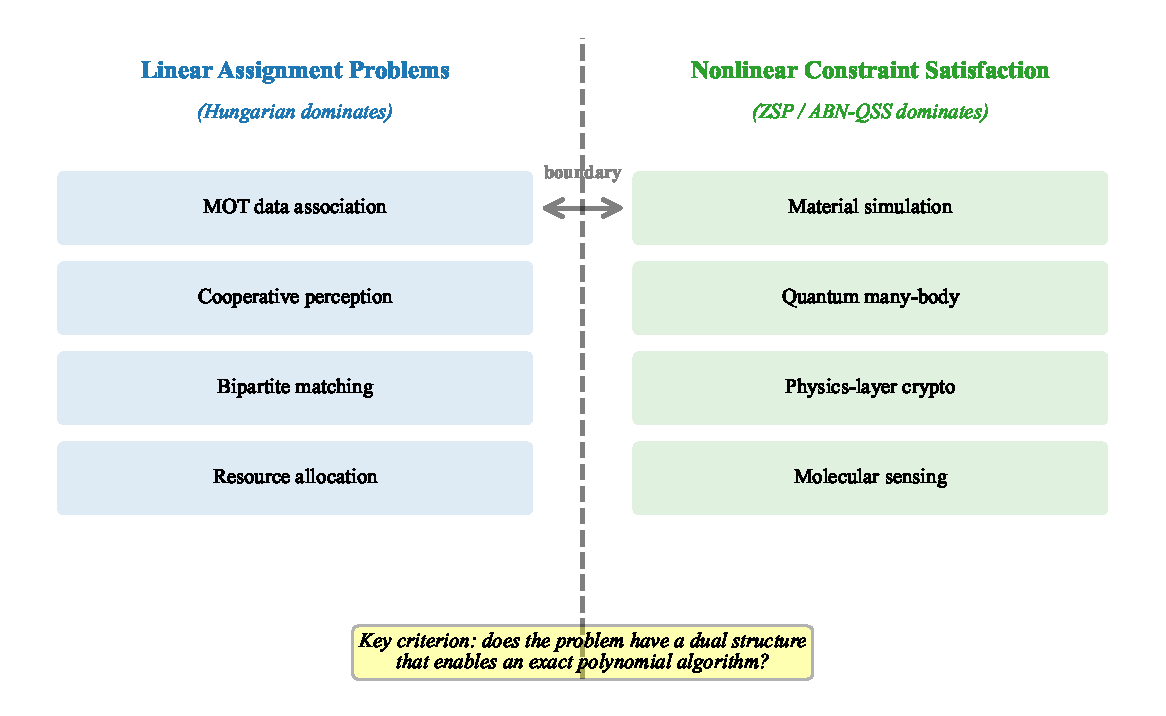
\includegraphics[width=0.85\linewidth]{figures/fig8_boundary.pdf}
    \caption{Applicability boundary of \ZSP. Problems with dual 
    structure (left) are best solved by exact polynomial algorithms. 
    Problems without such structure (right) are the natural domain 
    of \ZSP.}
    \label{fig:boundary}
\end{figure}

\begin{table}[t]
    \centering
    \caption{Where \ZSP helps and where it doesn't.}
    \label{tab:applicability}
    \begin{tabular}{l c c}
        \toprule
        Problem class & Dual structure? & \ZSP suitable? \\
        \midrule
        Linear assignment (\MOT, cooperative) & Yes & No \\
        Non-convex constraint satisfaction & No & Yes \\
        Physics field simulation & No & Yes \\
        High-dim non-linear optimization & No & Yes \\
        \bottomrule
    \end{tabular}
\end{table}

As \cref{tab:applicability} shows, \ZSP is well-suited for problems 
that lack a dual structure and thus lack exact polynomial algorithms.

\subsection{Implications for Physics-Native Computing}

The original application targets of \abnqss v3.0 are:
\begin{itemize}[leftmargin=*]
    \item \textbf{Material simulation}: entanglement fingerprint 
          analysis via Hadamard grid projection.
    \item \textbf{Secure communication}: physical-layer error 
          correction via $M C = 0$ constraints.
    \item \textbf{High-precision sensing}: molecular detection via 
          locked linearity.
    \item \textbf{Field solving}: variational relaxation for 
          high-dimensional PDEs.
\end{itemize}
These problems either lack or are not well-served by exact 
polynomial algorithms. This is where \ZSP's iterative nature becomes 
an \emph{advantage}---the physics itself performs the iteration in 
parallel, at speeds no digital computer can match.

\subsection{Why the Negative Result Matters}

Negative results are underexplored in machine learning and 
computing research. They have unique value:
\begin{enumerate}[leftmargin=*]
    \item \textbf{Boundary mapping}: they delineate what a method 
          cannot do, saving future researchers from repeating 
          the same dead ends.
    \item \textbf{Theory validation}: they confirm theoretical 
          predictions (here, LP duality) in practice.
    \item \textbf{Resource reallocation}: they redirect effort 
          toward problems where the method has an advantage.
\end{enumerate}

\subsection{Future Directions}

Based on our analysis, we recommend:
\begin{enumerate}[leftmargin=*]
    \item \textbf{Material simulation}: implement the Hadamard 
          grid for entanglement fingerprinting.
    \item \textbf{Physics-layer cryptography}: prototype the 
          PUF / limit-cycle key agreement.
    \item \textbf{FPGA mapping}: convert the digital twin to 
          Verilog-A / SPICE netlists.
    \item \textbf{Silicon photonics tape-out}: partner with 
          a foundry for 40nm CMOS + SOI MPW.
\end{enumerate}